\documentclass{beamer}
\usepackage[utf8]{inputenc}
\usepackage{amsmath, amssymb}
\usepackage{bbm}
\usepackage{dsfont}
\usepackage{hyperref}
\usepackage{tabularx}
\usepackage{booktabs}
\usepackage{multirow}
\hypersetup{hidelinks}

\usepackage{multirow}
% Packages
\usepackage{biblatex}
\usetheme{Madrid}
\setbeamerfont{normal text}{size=\small}
% disable the fancy (usually dark) styling and use a simple rounded style:
\setbeamertemplate{blocks}[rounded][shadow=false]

% make all block‐titles light blue:
\setbeamercolor{block title}{fg=black,bg=blue!20}
\setbeamercolor{block body}{fg=black,bg=blue!5}

% if you still want an 'alertblock' but in light yellow:
\setbeamercolor{alertblock title}{fg=black,bg=yellow!40}
\setbeamercolor{alertblock body}{fg=black,bg=yellow!10}
\title{Analysis of spatially clustered survival data with unobserved covariates using SBART}
\author{Durbadal Ghosh}
\date{\today}

%%%%%%%%%%%%%%%%%%%%%%%%%%%%%%%%%%%%%%%%%%%%%%%%%%%%%%%%%%%%%%
\begin{document}


%%%%%%%%%%%%%%%%%%%%%%%%%%%%%%%%%%%%%%%%%%%%%%%%%%%%%%%%%%%%%%
\begin{frame}
  \titlepage
\end{frame}
%%%%%%%%%%%%%%%%%%%%%%%%%%%%%%%%%%%%%%%%%%%%%%%%%%%%%%%%%%%%%%
\begin{frame}
  \tableofcontents
\end{frame}

%%%%%%%%%%%%%%%%%%%%%%%%%%%%%%%%%%%%%%%%%%%%%%%%%%%%%%%%%%%%%%





\section{Chapter 1: NP Bayes analysis of spatially clustered survival data with unobserved covariates}
\begin{frame}{}
    \centering
    \textbf{Chapter 1: NP Bayes analysis of spatially clustered survival data with unobserved covariates}
\end{frame}
\subsection{Motivation}

\begin{frame}{FL Cancer Registry}
\protect\hypertarget{motivating-dataset}{}
\begin{itemize}
\vfill \item
  Breast cancer patients in FL: FCR study
\vfill \item
  Survival Response: Time to death (right censored)
\vfill \item
   Clusters (K=67): FL Counties
\vfill \item 2 Races: African American (AA) / Non-African American (WA)
\vfill \item
  5 patient-level covariates
%\vfill \item Goal: Effects of covariates on racial disparity
\pause
\vfill \item Challenge: Covariate \textcolor{blue}{Mammography-Screening (SMU)} not in the registry!
%\vfill \item Augment from another study (BRFSS)
\pause
\vfill \item \textcolor{blue}{SMU ($\mathbf{M}$)}: a parameter in BRFSS study

\vfill \item Goal: $\mathbf{x, \textcolor{blue}{M}}$ $\longrightarrow\ P[T>t\mid \mathbf{x, \textcolor{blue}{M}}]=S(t|\mathbf{x, \textcolor{blue}{M}})$
\end{itemize}
\end{frame}
%%%%%%%%%%%%%%%%%%%%%%%%%%%%%%%%%%%%%%%%%%%%%%%%%%%%%%%%%%%%%%

\begin{frame}{Challenges}
\protect\hypertarget{challenges}{}
\begin{itemize}
\vfill \item
  Right Censored Survival data
\vfill \item
  Clustered survival with variable cluster sizes
\vfill \item
  Spatial association among cluster effects

\vfill \item
\textcolor{blue}{Unobserved county-level SMU}

\vfill \item
  Spatial association among \textcolor{blue}{unobserved SMU values}

\medskip

\vfill \item
 Semiparametric models: not valid

\vfill \item Unknown interactions/forms of covariates $\mathbf{X}$

\vfill \item Need: nonparametric modeling of risk/hazard


\vfill \item 
  Computational Challenges
\end{itemize}
\end{frame}

%%%%%%%%%%%%%%%%%%%%%%%%%%%%%%%%%%%%%%%%%%%%%%%%%%%%%%%%%%%%%%


\begin{frame}{}
\includegraphics[width=1.04\textwidth]{pics/Flowchart.png}
    FCR: $\mathcal{D}_1=\{y_{ij},\delta_{ij},\mathbf{x}_{ij}\}$  and   BRFSS: $\mathcal{D}_0=(D_{01},\cdots,D_{0K})$
\end{frame}

%%%%%%%%%%%%%%%%%%%%%%%%%%%%%%%%%%%%%%%%%%%%%%%%%%%%%%%%%%%%%%
%%%%%%%%%%%%%%%%%%%%%%%%%%%%%%%%%%%%%%%%%%%%%%%%%%%%%%%%%%%%%%
\subsection{Submodels}


% \begin{itemize}
%   \vfill  \item $\textcolor{blue}{\mathbf{M}}\sim \text{MVN}(\mathbf{0},\sigma_0^2(\mathbf{D}-\rho_0 \mathbf{A})^{-1})$ 
%     \item $\rho_0 \in (\frac{1}{\alpha_1},\frac{1}{\alpha_n})$ 
%    \vfill \item  $\alpha_1$: Minimum eigenvalue of $\mathbf{A}$
%    \vfill \item  $\alpha_n$: Maximum eigenvalue of $\mathbf{A}$
%    \vfill \item $\boldsymbol{\eta}_0=(\rho_0,\sigma_0)$
%    \vfill \item $\text{CAR}(\boldsymbol{\eta}_0):=\text{MVN}(\mathbf{0},\sigma_0^2(\mathbf{D}-\rho_0 \mathbf{A})^{-1})$
% \end{itemize}
% \end{frame}
%%%%%%%%%%%%%%%%%%%%%%%%%%%%%%%%%%%%%%%%%%%%%%%%%%%%%%%%%%%%%%
%\subsubsection{Submodel for Survival}
\begin{frame}{Notation}
\protect\hypertarget{notation}{}
\begin{itemize}
\vfill \item
  Clusters \(i= 1,2,...,K\); Patients \(j = 1,2,...,n_i\) 
\vfill \item
  Survival Time: \(T_{ij}\); Censoring: \(C_{ij}\)
\vfill \item 
   Observed survival: \(Y_{ij}= Min\{C_{ij},T_{ij}\} \)
   
   \vfill \item Censoring
  Indicator: \(\delta_{ij}\)

\vfill \item
  Covariates:
  \(\mathbf{x}_{ij} \in \mathbb{R}^p\) 
\vfill \item
  Survival data: 
  \(\mathcal{D}_1= \{(y_{ij},\delta_{ij};\mathbf{x}_{ij})  \}\)
  
\vfill \item
  Survival function:
  \(S_{ij}(t| \mathbf{x}_{ij},\textcolor{blue}{M_i})= P(T_{ij}>t|\mathbf{x}_{ij},\textcolor{blue}{M_i})\)
\vfill \item
  Hazard function:
  \(\lambda_{ij}(t|\mathbf{x}_{ij},\textcolor{blue}{M_i})\)
  % =\frac{f(t|\mathbf{x}_{ij},\textcolor{blue}{M_i})}{S(t|\mathbf{x}_{ij},\textcolor{blue}{M_i})}\)
\end{itemize}
\end{frame}
%%%%%%%%%%%%%%%%%%%%%%%%%%%%%%%%%%%%%%%%%%%%%%%%%%%%%%%%%%%%%%
\begin{frame}{Key Modeling Features}
\begin{itemize}
\vfill \item
  \(\lambda_{ij}(t| W_i,\textcolor{blue}{M_i};\mathbf{x}_{ij}) = \lambda_0 \ W_i\  \Phi(b(t, \textcolor{blue}{M_i},\mathbf{x}_{ij}))\) 
  % \vfill \item $\Phi$: CDF of Standard Normal Distribution
   \vfill \item  $b(t,\textcolor{blue}{M_i};\mathbf{x}_{ij}): \mathbb{R}^+ \times [0,1]\times \mathbb{R}^{p} \to \mathbb{R}$
  \vfill \item
  \(\lambda_0\): Constant baseline hazard 
  \vfill \item \textcolor{blue}{$M_i$}: Unobserved SMU
\vfill \item
  \(W_i\): Unobserved county effect
\vfill \item \(\mathbf{W}=(W_1,\cdots,W_K)\): Spatially associated
\vfill \item $L_{1ij}(W_i, \lambda_0,b; \textcolor{blue}{M_i})$: Likelihood contribution of $(i,j)$ 

% \vfill \item
%   \(log(\mathbf{W}) \sim CAR(\boldsymbol{\eta}_1)\)
 

   
%   \vfill\item Likelihood Contribution of $(i,j)$:

% $L_{1ij}(W_i, \lambda_0,b; \textcolor{blue}{M_i})\propto \{\lambda_0 W_i\Phi(b(y_{ij}, \textcolor{blue}{M_i}; \mathbf{x}_{ij}))\}^{\delta_{ij}}
% \ \exp\left\{-W_i \ \lambda_0  \int_0^{y_{ij}}\ \Phi(b(s,\textcolor{blue}{M_i},\mathbf{x}_{ij})) \ ds\right\}\ 
% $
\end{itemize}    
    
\end{frame}
\begin{frame}{Conditional Auto-Regressive model (CAR) for $\mathbf{W}$}
\protect\hypertarget{conditional-auto-regressive-model-car}{}
\begin{itemize}
\vfill \item
  Areal data: only county locations
\vfill \item
  Neighboring counties should exhibit higher association



\vfill \item 
$E[\log {W}_i \mid \log {W}_{(-i)}] = \frac{\sum_{j \neq i}^{n} {A}_{ij} \log{W}_j}{\sum_{j \neq i}^{n} {A}_{ij}}.$
\pause

    % \vfill \item \(M_i\) : cluster effect of county \(i\)
    
   % \vfill \item \({A}_{ij}\): Spatial distance/weights between clusters \(i\) and \(j\)

   \vfill \item $\mathbf{W}\sim \text{CAR}(\boldsymbol{\eta}_1):=\text{MVN}(\mathbf{0},\sigma_1^2(\mathbf{D}-\rho_1 \mathbf{A})^{-1})$
       
     \vfill \item $\boldsymbol{\eta}_1=(\rho_1,\sigma_1)$
   \vfill \item \(\mathbf{A}\): Adjacency matrix for counties in FL
     \vfill  \item $\mathbf{D}=\operatorname{diag}(A_{1+},A_{2+} \cdots A_{K+})$, and $ A_{i+}=\sum_{j = 1}^K A_{ij}$
\end{itemize}
\end{frame}

\begin{frame}{Priors for Survival Model}
\protect\hypertarget{model-using-sbart}{}
\begin{itemize}
% \vfill \item
%   \(\lambda_{ij}(t| W_i,\textcolor{blue}{M_i};\mathbf{x}_{ij}) = \lambda_0 \ W_i\  \Phi(b(t, \textcolor{blue}{M_i},\mathbf{x}_{ij}))\) 
  % \vfill \item $\Phi$: CDF of Standard Normal Distribution
  \vfill \item $\sigma_1 \sim \text{InvGamma}(a_{\sigma_1},b_{\sigma_1})$
  \vfill \item  $\rho_1 \sim \text{Uniform}(\frac{1}{\alpha_1},\frac{1}{\alpha_n})$ 
 \vfill \item \(\lambda_0 \sim \text{Gamma}(a_{\lambda},b_{\lambda})\)  
  
% \vfill \item
%   \(W_i\): County effect

% \vfill \item
%   \(log(\mathbf{W}) \sim CAR(\boldsymbol{\eta}_1)\)
 

    \vfill \item  SBART prior on $b(\cdot)$


\end{itemize}    


% \alert{Posterior of $b$: analytically intractable \& computationally expensive!}
\end{frame}
% \subsection{Review of BART and SBART}
\begin{frame}{Bayesian Additive Regression Trees (BART)}
\protect\hypertarget{review-of-bayesian-additive-regression-trees-bart}{}
\begin{itemize}

\vfill \item
  \(b:\mathbb{R}^p \to \mathbb{R}\) unknown regression function
  \vfill \item
  Example: 1. Continuous response: $y \sim N(b(\mathbf{x}),1)$
   \\ 2. Binary response: $y \sim Ber(\Phi(b(\mathbf{x})))$
% \vfill \item
%   \(y=b(\mathbf{x})+\epsilon\) with \(\mathbf{x} \in \mathbb{R}^p\)
%   and \(\epsilon \sim N(0,\sigma^2_\epsilon)\)  
\vfill \item
  \(b(\cdot) = \sum_{h=1}^{H}g(\cdot; \mathcal{T}_h, \mathcal{M}_h)\)

    \(\mathcal{T}_h\) : topology and splitting rules of tree \(h\)

    \(\mathcal{M}_h = (\mu_{h1}, \dots, \mu_{h\mathcal{M}_h})\): predictions associated with terminal nodes
\end{itemize}
\end{frame}
\begin{frame}{Decision Trees}
\protect\hypertarget{review-of-bart}{}
\begin{center}\includegraphics[width=.9\textwidth]{figures/Treefigsinhappt.png} \end{center}
\end{frame}
%%%%%%%%%%%%%%%%%%%%%%%%%%%%%%%%%%%%%%%%%%%%%%%%%%%%%%%%%%%%%%
\begin{frame}{Decision Tree, Partitions and Leaves}
\protect\hypertarget{an-example-of-partition-due-tree}{}
\alert{\(b(\mathbf{x})\) : piece-wise constant over all partitions of $\mathcal{X}$}
\begin{center}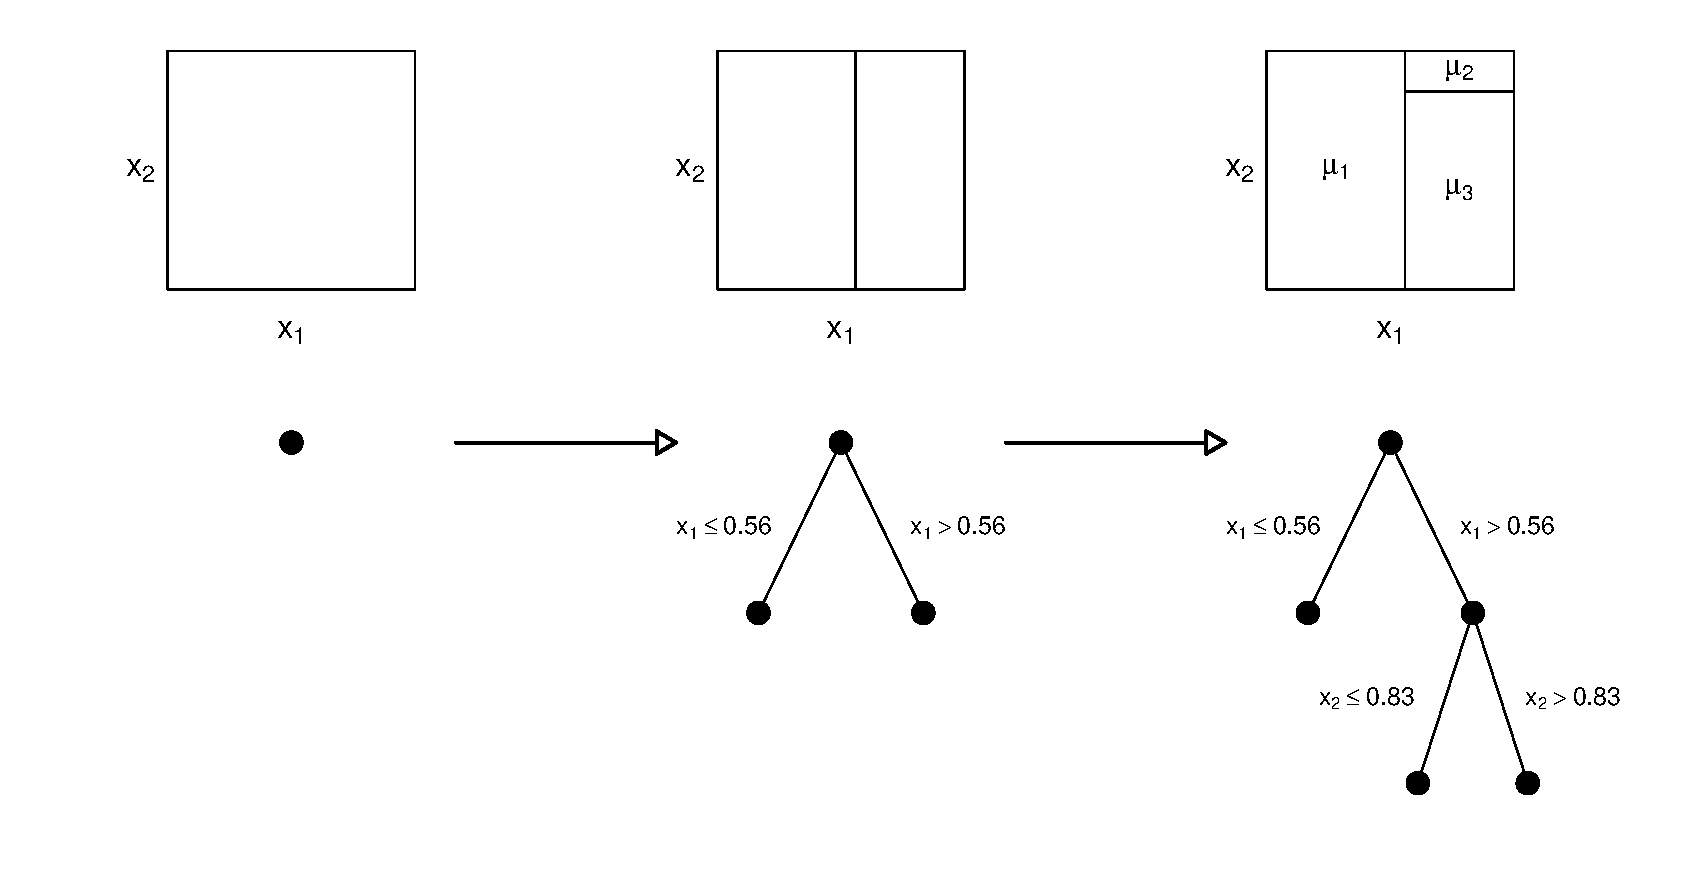
\includegraphics[width=.8\textwidth]{figures/BARTdiagram.eps} \end{center}

Fast computation using  Backfitting  
\\ R packages: SoftBART, BART, bartMachine
\end{frame}
%%%%%%%%%%%%%%%%%%%%%%%%%%%%%%%%%%%%%%%%%%%%%%%%%%%%%%%%%%%%%%
\begin{frame}{BART and SBART}
\protect\hypertarget{bart-and-sbart}{}
\includegraphics[width=0.49\textwidth]{figures/partition1.eps}
\includegraphics[width=0.49\textwidth]{figures/Partition2.eps}
\vfill Left: BART, Right: SBART
\end{frame}



%\subsubsection{Unobserved covariate $M$}
\begin{frame}{Submodel for the cluster-level SMU}
\protect\hypertarget{estimation-error-in-cluster-level-covariate-smu}{}
\begin{itemize}
\vfill \item
\textcolor{blue}{True/unobserved SMU:} Spatial association. 
\end{itemize}

\begin{itemize}
% \vfill \item $\mathcal{D}_0=(D_{01},\cdots,D_{0K})$ from BRFSS
 \vfill \item $D_{0i}=(n_{0i},m_{0i})$ from BRFSS
    
    \vfill \item \textcolor{blue}{\( M_i\):} ``True" \textcolor{blue}{SMU proportion} for county \(i\)
\end{itemize}


\textbf{Likelihood from BRFSS}: \[ L_{0i}(\textcolor{blue}{M_i}\mid D_{0i}): \quad m_{0i} \sim Binom(n_{0i},\textcolor{blue}{M_i})\]

\textbf{Distribution of} $\textcolor{blue}{\mathbf{M}}$: \[\text{logit}(\textcolor{blue}{\mathbf{M}})\sim
CAR(\boldsymbol{\eta}_0)
\]
\end{frame}
%%%%%%%%%%%%%%%%%%%%%%%%%%%%%%%%%%%%%%%%%%%%%%%%%%%%%%%%%%%%%%
%%%%%%%%%%%%%%%%%%%%%%%%%%%%%%%%%%%%%%%%%%%%%%%%%%%%%%%%%%%%%%
% \begin{frame}{Conditional Auto-Regressive model (CAR)}
% \protect\hypertarget{conditional-auto-regressive-model-car}{}
% \begin{itemize}
% \vfill \item
%   Areal data: only county locations
% \vfill \item
%   Neighboring counties should exhibit higher association



% \vfill \item 
% $E[\text{logit}(\textcolor{blue}{M}_i) \mid \text{logit}(\textcolor{blue}{M}_{(-i)})] = \frac{\sum_{j \neq i}^{n} {A}_{ij} \text{logit}(\textcolor{blue}{M}_j)}{\sum_{j \neq i}^{n} {A}_{ij}}.$

%     % \vfill \item \(M_i\) : cluster effect of county \(i\)
    
%    % \vfill \item \({A}_{ij}\): Spatial distance/weights between clusters \(i\) and \(j\)
%     \vfill \item \(\mathbf{A}\): Adjacency matrix for counties in Fl
%      \vfill  \item $\mathbf{D}=\operatorname{diag}(A_{1+},A_{2+} \cdots A_{K+})$, and $ A_{i+}=\sum_{j = 1}^K A_{ij}$
%      \vfill \item $\boldsymbol{\eta}_0=(\rho_0,\sigma_0)$
%    \vfill \item $\text{CAR}(\boldsymbol{\eta}_0):=\text{MVN}(\mathbf{0},\sigma_0^2(\mathbf{D}-\rho_0 \mathbf{A})^{-1})$
% \end{itemize}
% \end{frame}
%%%%%%%%%%%%%%%%%%%%%%%%%%%%%%%%%%%%%%%%%%%%%%%%%%%%%%%%%%%%%%
% \begin{frame}{CAR model}
% \begin{itemize}

%   \vfill  \item $\textcolor{blue}{\mathbf{M}} \sim \text{MVN}(\mathbf{0},\sigma_0^2(\mathbf{D}- \mathbf{A})^{-1})$ (Gaussian Markov random field)
% \end{itemize}

% \vfill \alert{Improper Distribution!}


%%%%%%%%%%%%%%%%%%%%%%%%%%%%%%%%%%%%%%%%%%%%%%%%%%%%%%%%%%%%%%



% \begin{frame}[label=data-augmentation]{Data Augmentation}

%   \alert{Challenge: Sampling \(\theta\) from \(f(\theta \mid \mathcal{D})\) is difficult!}

%   \begin{alertblock}{Data Augmentation}
%     Find a “latent” \(Z^*\) such that both
%     \[
%       \theta \sim f(\theta \mid Z^*, \mathcal{D})
%       \quad\text{and}\quad
%       Z^* \sim f(Z^* \mid \theta, \mathcal{D})
%     \]
%     are straightforward to sample.
%   \end{alertblock}

%   \begin{block}{Gibbs–Style Sampling}
%     \begin{enumerate}
%       \item Sample \(Z^* \sim f(Z^* \mid \theta, \mathcal{D})\).
%       \item Sample \(\theta \sim f(\theta \mid Z^*, \mathcal{D})\).
%       \item \emph{Repeat} until convergence.
%     \end{enumerate}
%   \end{block}

% \end{frame}

%%%%%%%%%%%%%%%%%%%%%%%%%%%%%%%%%%%%%%%%%%%%%%%%%%%%%%%%%%%%%%


% \begin{frame}{Data augmentation scheme for no-censoring}
% \vspace{8pt}
% \vfill \begin{block}{Step 1}
% \[\mathbf{G}_{ij} \mid (y_{ij},b,\lambda_0,\textcolor{blue}{M_i},\mathbf{x}_{ij}) \sim NHPP [ \lambda_0 W_i \{1-\Phi (b(s,\textcolor{blue}{M_i},\mathbf{x}_{ij})\}] \]
% \quad \quad \quad for \(s \in (0,y_{ij})\)
% \medskip 

% Latent variables: $\mathbf{G}_{ij}=\{G_{ij1},..., G_{ijq_{ij}}\}$
% \end{block}
% \vfill \begin{block}{Step 2}
% \(\{\tilde{G}_{ijg}; g = 1,\ldots, q_{ij}+1\}\) such that \[
%   \tilde{G}_{ijg} \mid \mathbf{G}_{ij}, y_{ij} \sim
%   \begin{cases}
%     N(b(G_{ijg},\textcolor{blue}{M_i}, \mathbf{x}_{ij}),1)I(-\infty,0), & \text{if}\ g=1,\dots,q_{ij} \\
%     N(b(y_{ij},\textcolor{blue}{M_i}, \mathbf{x}_{ij}),1)I(0,\infty), & \text{if}\ g=q_{ij}+1.
%   \end{cases}
% \]
% \end{block}



% \footnotesize \textcolor{red}{Full Conditional: $\prod_{i,j,k}\phi(\tilde{G}_{ijk}\mid b(G_{ijk},\textcolor{blue}{M_i},\mathbf{x}_{ij});\ 1)] \times \Pi(\mathbf{b})$. Use standard packages}
% \end{frame}

%%%%%%%%%%%%%%%%%%%%%%%%%%%%%%%%%%%%%%%%%%%%%%%%%%%%%%%%%%%%%%
%\subsubsection{Combining the two models}



\begin{frame}{Combining the two models}
\begin{itemize} 
  \vfill \item \( \mathcal{D}_1\): FCR
 \vfill \item $\mathcal{D}_0$: BRFSS
  \vfill  \item The observed data  \(\mathcal{D}=\{\mathcal{D}_0,\mathcal{D}_1\}\)
\vfill \item \textbf{Posterior}  
\[\propto 
[\prod_{i=1}^K\{\prod_{j=1}^{n_i} L_{1ij}\}]  L_0(\textcolor{blue}{\mathbf{M}}|\mathcal{D}_0) g_1(\mathbf{W} \mid \boldsymbol{\eta}_1) g_0(\textcolor{blue}{\mathbf{M}} \mid \boldsymbol{\eta}_0)  p(b \mid \boldsymbol{\Psi}_1)  p(\lambda_0)  p(\boldsymbol{\Omega}) \]
\vfill \item \(\boldsymbol{\Omega}=\{\boldsymbol{\eta}_0,\boldsymbol{\eta}_1,\boldsymbol{\Psi}_1\}\)

   \vfill \item The major challenge: \textcolor{red}{presence of $\mathbf{M}$ in both $\prod_{(i,j)} L_{1ij}$ and $L_0$.} 
\end{itemize}  
\end{frame}
%%%%%%%%%%%%%%%%%%%%%%%%%%%%%%%%%%%%%%%%%%%%%%%%%%%%%%%%%%%%%%
\begin{frame}{The three-stage method}
\begin{itemize}
    \vfill \item \textbf{Step~1}: Obtain samples of \(\textcolor{blue}{\mathbf{M}}\) from 
    \[ \left[(\textcolor{blue}{\mathbf{M}},\boldsymbol{\eta}_0\vert \mathcal{D}_0]\propto [L_0(\textcolor{blue}{\mathbf{M}}|\mathcal{D}_0)\right]\times g_0(\textcolor{blue}{\mathbf{M}}|\boldsymbol{\eta}_0)\times p(\boldsymbol{\eta}_0)\] 
    and compute \(\hat{\textcolor{blue}{\mathbf{M}}}=\operatorname{E}[\textcolor{blue}{\mathbf{M}}\mid \mathcal{D}_0]\)
    
    
    \vfill \item \textbf{Step~2}: Obtain MCMC samples of $\{b,\lambda_0,\boldsymbol{\eta}_1,\boldsymbol{\Psi}_1\}$ and $\mathbf{W}$ from 
\[\propto 
[\prod_{i=1}^K\{\prod_{j=1}^{n_i} L_{1ij}(W_i,\lambda_0,b;\textcolor{blue}{\hat{M}_i})\}] g_1(\mathbf{W} \mid \boldsymbol{\eta}_1) p(b \mid \boldsymbol{\Psi}_1) p(\lambda_0)p(\boldsymbol{\Psi}_1) p(\boldsymbol{\eta}_1)\ 
\]

\vfill \item \textbf{Step~3}: Use samples as \textcolor{red}{importance samples} with weights 
\[\propto \prod_{i=1}^K[\prod_{j=1}^{n_i}\{ L_{1ij}(W_i,\lambda_0,b;\textcolor{blue}{M_i})/ L_{1ij}(W_i,\lambda_0,b;\textcolor{blue}{\hat{M}_i})\}]\]
\end{itemize}
\end{frame}
%%%%%%%%%%%%%%%%%%%%%%%%%%%%%%%%%%%%%%%%%%%%%%%%%%%%%%%%%%%%%%




% \begin{frame}{Innovations in Computations}
% \protect\hypertarget{computation}{}
% \begin{itemize}
% \vfill\item Data Augmentation for Gibbs sampling and simplified importance weighting

% \vfill\item Importance sampling to connect two models

% \vfill\item Hamiltonian Monte Carlo for frailty updates (many clusters)
  
% \vfill\item R-Stan interface and SoftBART package
% \end{itemize}
% \end{frame}


%%%%%%%%%%%%%%%%%%%%%%%%%%%%%%%%%%%%%%%%%%%%%%%%%%%%%%%%%%%%%%


%%%%%%%%%%%%%%%%%%%%%%%%%%%%%%%%%%%%%%%%%%%%%%%%%%%%%%%%%%%%%%





\subsection{Simulation Study}



\begin{frame}{Simulation Results}

\begin{itemize}
    \vfill \item \textbf{Simulation A}: $\lambda_{ij}(t| W_i,\textcolor{blue}{M_i};x_{1ij},x_{2ij})= W_i \exp(t x_{1ij}+ 0.25x^2_{1ij}+0.5\textcolor{blue}{M_i})$. 
    \vfill \item \textbf{Simulation B}: $\lambda_{ij}(t| W_i,\textcolor{blue}{M_i};x_{1ij},x_{2ij})= \exp(t x_{1ij} W_i+ 0.25x^2_{1ij}+0.5\textcolor{blue}{M_i})$. 
    \vfill \item \textbf{Simulation C}: $\lambda_{ij}(t| W_i,\textcolor{blue}{M_i};x_{1ij},x_{2ij})= W_i\exp(t x_{1ij}+ 0.25x^2_{1ij}+0.5\textcolor{blue}{M_i})$ where $\textcolor{blue}{M_i}=\frac{W_i}{1+W_i}$.
\end{itemize}


\textbf{AMSE of Survival Curves: }
\begin{table}[ht]
\centering

\resizebox{\columnwidth}{!}{
\begin{tabular}{rrrr}
  \hline
 & SIMULATION A & SIMULATION B & SIMULATION C \\ 
  \hline
Our Method & 0.25 & 0.11 & 0.19 \\ 
  COX-PH with frailty (Hougard) & 0.26 & 0.15 & 0.34 \\ 
  Random forest & 0.49 & 0.43 & 0.48 \\ 
   \hline
\end{tabular}
}





\end{table} 
%\begin{figure}[htbp]
%\includegraphics[height=.5\textheight]{SIM_A.eps}
%\caption{Estimated Survival Curves for different values of covariates in each of 3 simulation scenarios. The black curve represents the true Survival Function, the green curve is the estimated survival curve estimated by our method, the red curve is the estimated survival curve estimated by Random Survival Forest, and the blue curve is the estimated survival curve estimated by Cox's proportional hazard method.}
%\end{figure}


\end{frame}
% \begin{frame}{Survival Curves for Simulation A}
%     \begin{figure}
%         \centering
%         \includegraphics[height=.7\linewidth]{figures/SIM_A.pdf}
        
%         \label{fig:enter-label}
%     \end{figure}
% \end{frame}


%%%%%%%%%%%%%%%%%%%%%%%%%%%%%%%%%%%%%%%%%%%%%%%%%%%%%%%%%%%%%%
\subsection{Data Analysis}

% \begin{frame}{Study Description}

% \textbf{Strata; Clusters; Covariates:} 
%     \begin{itemize}
%         \vfill \item Race: African American / Non African American
%         \vfill \item Stage at diagnosis: Distant / Regional / Local
%         \vfill \item 6 strata: 3 stages $\times$ 2 races
%         \vfill \item County: cluster
%         \vfill \item HR Status: Negative / Positive
%         \vfill \item Tumor Grade: 1 / 2 / 3
%         \vfill \item Age: Continuous
%         \vfill \item Biopsy Delay: Long / Short
%         \vfill \item Treatment Delay: Long / Short
%         \vfill \item \textcolor{blue}{Screening Mammography: SMU (unobserved)}
%     \end{itemize}


% \end{frame}
\begin{frame}{Analysis goals}

\begin{itemize}
   \vfill \item Expected life years saved in 5 or 10 years
    % \vfill \item Estimate $\int_{0}^{10} [S_T(t | \mathbf{x}^*) - S_T(t | \mathbf{x}_{obs})] dt$ 
    % \vfill \item $\mathbf{x}_{obs}$: covariates of an ``average" patient
    % \vfill \item $\mathbf{x}^*$: covariate values after mitigating disparity
    \vfill \item  Relative importance of a covariate in survival?
    \vfill \item Effect of Treatment Delay (1/0) on T?
    \vfill \item Effect of Biopsy Delay (1/0) on T?
    \vfill \item  Effect of \textcolor{blue}{SMU} (continuous)?
    \vfill \item  Which counties have more expected life years saved?
\end{itemize}

\end{frame}
%%%%%%%%%%%%%%%%%%%%%%%%%%%%%%%%%%%%%%%%%%%%%%%%%%%%%%%%%%%%%%
\begin{frame}{Importance of Covariates}
\protect\hypertarget{importance-of-covariates}{}
\renewcommand{\arraystretch}{1.2}
%\alert{We do a stratified analysis for each stage-race combination. There are three stages and two races, so there are six strata.}
\begin{table}[ht]
\centering

\begin{tabular}{rrrrrrr}
  \hline
& AA & AA  & AA & AW & AW & AW \\ 
 & Local & Region.  & Distant & Local & Region  & Distant \\
  \hline
Age & 0.113 & 0.155 & 0.149 & \textcolor{green}{0.175} & \textcolor{green}{0.171} & \textcolor{red}{0.162} \\ 
  HR Status & 0.163 & \textcolor{green}{0.166} & 0.103 & 0.143 & 0.143 & \textcolor{green}{0.170} \\ 
  Grade2 & 0.135 & 0.136 & 0.142 & 0.132 & 0.128 & 0.126 \\ 
  Grade3 & 0.135 & 0.115 & 0.138 & 0.146 & \textcolor{red}{0.159} & 0.134 \\ 
  \textcolor{blue}{SMU}  & \textcolor{green}{0.169} & 0.144 & \textcolor{green}{0.165} & 0.116 & 0.131 & 0.132 \\ 
  Tr. Delay & \textcolor{red}{0.163} & 0.127 & \textcolor{red}{0.157} & \textcolor{red}{0.149} & 0.136 & 0.132 \\ 
  Bio. Delay & 0.121 &\textcolor{red}{0.157} & 0.146 & 0.138 & 0.133 & 0.144 \\ 
   \hline
   

\end{tabular}


\end{table}
\begin{itemize}
    \item \textcolor{green}{Green:} Most important
    \item \textcolor{red}{Red:} Second Most important
\end{itemize}
%
%\begin{block}\textbf{Important intervene-able covariates :Racial
%Disparity}
%\protect\hypertarget{important-intervene-able-covariates-racial-disparity}{}
%\begin{itemize}
%\tightlist
%\vfill \item
 % \alertb{SMU}: Stage L and Stage D
%\vfill \item
 % \alertb{Biopsy Delay}: Stage R
%\end{itemize}
%\end{block}

\end{frame}

%%%%%%%%%%%%%%%%%%%%%%%%%%%%%%%%%%%%%%%%%%%%%%%%%%%%%%%%%%%%%%
\begin{frame}{Estimation of Survival Curve}
\protect\hypertarget{estimation-of-survival-function}{}
\begin{center}\includegraphics[width=1\textwidth]{figures/Survival_Curves_Based_Median_both_races.eps} \end{center}

\end{frame}
%%%%%%%%%%%%%%%%%%%%%%%%%%%%%%%%%%%%%%%%%%%%%%%%%%%%%%%%%%%%%%
\begin{frame}{Expected life years saved}

\protect\hypertarget{results}{}



\textbf{Life years (within 10 years) saved for an AA patient in ``Broward" county by mitigating racial disparities in the covariates}
\begin{table}
\centering

\begin{tabular}{l|c|c|c} 
\toprule
Intervenable & Tumor & \multicolumn{2}{c}{\underline{Cancer Stage}} \\

Covariate & Grade & Regional  & Distant \\
\midrule
\textcolor{blue}{SMU} & 1 &0.12 (0.11, 0.12) & 0.42 (0.41, 0.42) \\
& 2 & 0.16 (0.14, 0.16) & 0.40 (0.39, 0.43) \\
& 3 & 0.00 (0.00, 0.00) & 0.53 (0.52, 0.54) \\
\midrule
Biopsy Delay & 1 & 0.00 (0.00, 0.00) & 0.64 (0.64, 0.66) \\
& 2 & -0.01 (-0.02, 0.01) &0.65 (0.64, 0.67) \\
& 3 & -0.11 (-0.11, -0.09) & 0.75 (0.73, 0.78) \\
\midrule
Treatment Delay & 1 &0.84 (0.84, 0.84) & 0.59 (0.59, 0.59) \\
& 2 & 0.73 (0.72, 0.75) & 0.50 (0.47, 0.50)\\
& 3 & 0.81 (0.81, 0.85) & 0.58 (0.56, 0.61) \\
\bottomrule
\end{tabular}
\end{table}
\end{frame}



\begin{frame}{County-wise Life Years Saved}
\includegraphics[width=.8\textwidth]{figures/Fl_map2.pdf}
    
\end{frame}

%%%%%%%%%%%%%%%%%%%%%%%%%%%%%%%%%%%%%%%%%%%%%%%%%%%%%%%%%%%%%%
% \begin{frame}{Summary}
% \protect\hypertarget{innovations}{}


% \begin{itemize}

% \vfill \item
%   Modeling continuous survival response with censoring

% \vfill \item NP model of risk/hazard  using SBART 




 
% \vfill \item
%   Spatially correlated cluster effects (frailties) on hazard and spatially correlated \textcolor{blue}{unobserved SMU}
  
% \vfill \item
%  Augmentation of \textcolor{blue}{unobserved SMU} 

%  \vfill \item Importance sampling technique to get unbiased estimates and a measure of uncertainty. 

 
% \medskip

% \vfill \item
%   Data Augmentation strategy for fast computation


% \vfill \item
%   Simulation


% \vfill \item Investigation of roles of covariates in racial disparity in each county
  
% \end{itemize}
% \end{frame}




%%%%%%%%%%%%%%%%%%%%%%%%%%%%%%%%%%%%%%%%%%%%%%%%%%%%%%%%%%%%%%

\section{Chapter 2: Estimation of cluster-specific causal effects on a  spatially associated survival data using SBART}

\subsection{Introduction}
\begin{frame}{Chapter 2}
    \textbf{Estimation of cluster-specific causal effects on a  spatially associated survival data using SBART}
\end{frame}

\begin{frame}{Florida Cancer Registry}
    \begin{itemize}
      \vfill \item \textbf{Data:}
      \begin{itemize}
        \vfill \item 68,009 breast cancer patients from 67 counties in FL
      %  \vfill \item 
        \vfill \item Time-to-death (right-censored)
        \vfill \item  Cancer Treatment: delay ($>$90 days, $z=0$) vs no delay ($z=1$)
      \end{itemize}
      \vspace{6pt}
      \vfill \item \textbf{Goal:}
      \begin{itemize}
        \vfill \item Estimate the causal effects of $Z$ in each county
        
        \end{itemize}
        \pause
        \vfill \item \textbf{Challenges:}
        \begin{itemize}

        \vfill \item Confounders: $\mathbf{x}_{ij}$
        \vfill \item Spatial associations among counties
        \vfill \item Censoring
      \end{itemize}
      \vspace{6pt}
      \vfill \item \textbf{Our Approach:}
      \begin{itemize}
        \vfill \item Bayesian non-parametric regression using SBART
        \vfill \item Interpretable modelling of spatial association 
      \end{itemize}
    \end{itemize}
    \end{frame}
%%%%%%%%%%%%%%%%%%%%%%%%%%%%%%%%%%%%%%%%%%%%%%%%%%%%%%%%%%%%%%
\begin{frame}{ Motivation }
    \begin{itemize}
      \vfill \item \textbf{Why Account for Clustering and Spatial association?}
      \begin{itemize}
        \vfill \item Patients within same county(cluster) share unobservable traits.
        \vfill \item Variation of clusters/counties $\rightarrow$ causal inference (Hu, 2022)
        \vfill \item Neighboring counties may share similar features.
        \vfill \item County-specific treatment effects are of interest.
      \end{itemize}
      % \vspace{6pt}
      % \vfill \item \textbf{Why BART?}
      % \begin{itemize}
      %   \vfill \item Useful for non-linear regression.
      %   \vfill \item Provides  uncertainty quantification
      %   \vfill \item Promising in estimating causal effects. (Hill, 2011)
      % \end{itemize}
    \end{itemize}
    \end{frame}
%%%%%%%%%%%%%%%%%%%%%%%%%%%%%%%%%%%%%%%%%%%%%%%%%%%%%%%%%%%%%%

\begin{frame}{Previous Works}

\textbf{Frequentist Causal Survival Methods}
\begin{itemize}
    %\item IPW approaches \textcolor{blue}{(Xie 2005, Cole 2004)}
    \item PS matching/IPW \textcolor{blue}{(Austin 2013, Cole 2004)}
\end{itemize}

% \textbf{Spatial Causal Methods}
% \begin{itemize}
%     \item Neighborhood smoothing \textcolor{blue}{(Schnell \& Papadogeorgou 2020)}
%     % \item Spatial PS matching \textcolor{blue}{(Davis 2019)}
%     % \item Case-control matching \textcolor{blue}{(Jarner 2002)}
% \end{itemize}

\textbf{Bayesian \& Tree-Based Methods}
\begin{itemize}
    \item PS as confounder \textcolor{blue}{(Rubin 1985, Zigler 2015)}
    \item  Random Survival Forest \textcolor{blue}{(Tabib 2020)}
    % \item BART for ITE \textcolor{blue}{(Hill 2011, Dorie 2019)}
    \item AFT-BART models \textcolor{blue}{(Henderson 2020)}
    \item riAFT-BART for clustered data \textcolor{blue}{(Hu 2022)}
    
    % \item Deep Learning methods \textcolor{blue}{(Cui 2023)}
\end{itemize}
\pause
\begin{alertblock}{Key Limitations}
\begin{itemize}
    \item \textbf{Limited works:} Causal effects inside cluster
    \item \textbf{No integration:} spatial + causal + survival
    \item \textbf{ riAFT-BART:} handles clustered data, NOT spatial association

\end{itemize}
\end{alertblock}

\end{frame}
%%%%%%%%%%%%%%%%%%%%%%%%%%%%%%%%%%%%%%%%%%%%%%%%%%%%%%%%%%%%%%

%%%%%%%%%%%%%%%%%%%%%%%%%%%%%%%%%%%%%%%%%%%%%%%%%%%%%%%%%%%%%%




\subsection{Methods}
\begin{frame}{Notation and Definitions}
  \begin{itemize}
    \vfill \item \(i = 1,\dots,K\): clusters; \(j = 1,\dots,n_i\): subjects; \(N = \sum_i n_i\)
    \vfill \item Treatment: \(Z_{ij} \in \{0,1\}\)
    \vfill \item Confounders: \(\mathbf{X}_{ij}\) 
    \vfill \item Cluster-specific Random effects: $W_i$ 
    \vfill \item Survival time: \(T_{ij}\), censoring time: \(C_{ij}\)
    \vfill \item \(Y_{ij} = \min(T_{ij}, C_{ij})\), \(\delta_{ij} = \mathds{1}(T_{ij} < C_{ij})\)
    \pause
    \vfill \item Counterfactual: \(T_{ij}(1), T_{ij}(0)\), \(C_{ij}(1), C_{ij}(0)\)
    \vfill \item Observed data in the available sample: $\{\mathbf{x}_{ij}, z_{ij}, y_{ij},\delta_{ij} \}$
  \end{itemize}
\end{frame}

%%%%%%%%%%%%%%%%%%%%%%%%%%%%%%%%%%%%%%%%%%%%%%%%%%%%%%%%%%%%%%


\begin{frame}{Causal Estimands}
\begin{itemize}
  \vfill \item \textbf{Counterfactual Survival Functions:}
\begin{itemize}
    \vfill \item \( S^{(z)}_{ij}(t \mid   \mathbf{x}_{ij}) = P(T_{ij}(z) \geq t \mid   \mathbf{x}_{ij}, \text{Cluster}=i) \)
    %\vfill \item \( S^{(z)}(t) = \mathbb{E}_{\mathbf{x}_{ij}, \mathbf{v}}[S^{(z)}(t \mid \mathbf{x}_{ij}, \mathbf{v})] \)
  \end{itemize}
  \vspace{6pt}
  \vfill \item \textbf{Conditional Estimands:}
  \begin{itemize}
   \vfill \item ${\text{CSPTE}}_{ij}(t \mid   \mathbf{x}_{ij} ) = S^{(1)}(t \mid   \mathbf{x}_{ij}, \text{Cluster}=i) - S^{(0)}(t \mid   \mathbf{x}_{ij}, \text{Cluster}=i)$
    
    \vfill \item $\text{CERM}_{ij}(t^*, \mathbf{x}_{ij}) = \mathbb{E}[\{T_{ij}(1) \wedge t^*\} - \{T_{ij}(0) \wedge t^*\} \mid   \mathbf{x}_{ij}, \text{Cluster}=i]$
    \end{itemize}
%     \vspace{6pt}
%   \vfill \item \textbf{County-specific Estimands:}
%   \begin{itemize}
%     \vfill \item  \( {\text{C-ATE}}_i = \frac{1}{n_i} \sum_{j=1}^{n_i} {\text{CATE}_i}(\mathbf{x}_{ij}, \mathbf{v}_{i}) \)
%     \vfill \item  \( {\text{A-CERM}}_i(t^*) = \frac{1}{n_i} \sum_{j=1}^{n_i} {\text{CERM}_i}(t^*, \mathbf{x}_{ij}, \mathbf{v}_{i}) \)
%     \vfill \item $\text{C-ATT}_i = \frac{1}{n_{1i}} \sum_{j: z_{ij}=1} \text{CATE}_i(\mathbf{x}_{ij}, \mathbf{v}_{i})$
% \end{itemize}
\end{itemize}
\end{frame}

%%%%%%%%%%%%%%%%%%%%%%%%%%%%%%%%%%%%%%%%%%%%%%%%%%%%%%%%%%%%%%



%%%%%%%%%%%%%%%%%%%%%%%%%%%%%%%%%%%%%%%%%%%%%%%%%%%%%%%%%%%%%%
\begin{frame}{Causal Models with key assumptions}
    \begin{enumerate}
\item \textbf{SUTVA:} 
\begin{equation}
   T_{ij}(z_{11},\cdots,z_{1n_1},\cdots z_{Kn_K}) = T_{ij}(z_{ij}),
   \hspace{2pt}
   \label{eq:SUTVA}
   \end{equation}


\item \textbf{Consistency:} 

\begin{equation}
   T_{ij} = T_{ij}(1)\ \mathds{1}(Z_{ij}=1)\ +\ T_{ij}(0)\ \mathds{1}(Z_{ij}=0)
   \hspace{2pt},
   \label{eq:Consistency_Outcome}
   \end{equation}
% The observed outcome and observed censoring time of any 
% subject are the same as the potential survival and the potential censoring time corresponding to  the allocated treatment, that is
%    \begin{equation}
%   \mathds{1}(Z_{ij}=0)
%    \hspace{2pt},
%    \label{eq:Consistency_Outcome}
%    \end{equation}

   \begin{equation}
   C_{ij} = C_{ij}(1)\ \mathds{1}(Z_{ij}=1)\ +\ C_{ij}(0)\ \mathds{1}(Z_{ij}=0)
   \hspace{2pt}.
   \label{eq:Consistency_Censor}
   \end{equation}
%   The observed outcome corresponds to the potential outcome under the treatment received.

\item \textbf{Unconfoundedness:}
\begin{equation}
  \left( T_{ij}(1), T_{ij}(0) \right) \perp\!\!\!\perp Z_{ij} \mid   \mathbf{X}_{ij}
   \end{equation}

% \item \textbf{Positivity:}    

%    \begin{equation}
%    0 <  P(Z_{ij}=1 \mid   \mathbf{X}_{ij}) < 1
%    \hspace{2pt}.
%    \label{eq:Positivity}
%    \end{equation}


% \item \textbf{Conditionally independent Censoring:} For $z \in \{0,1\}$  
%    \begin{equation}
%   \left( T_{ij}(1), T_{ij}(0) , W_i\right)  \perp\!\!\!\perp \left( C_{ij}(1), C_{ij}(0) \right)  \mid   \mathbf{X}_{ij}, Z_{ij} =z
%    \hspace{2pt}. 
%    \label{eq:IndCensoring}
%    \end{equation}
   
\end{enumerate}


\end{frame}
%%%%%%%%%%%%%%%%%%%%%%%%%%%%%%%%%%%%%%%%%%%%%%%%%%%%%%%%%%%%%%
 % \begin{frame}{Causal Graph}
 
 %     \includegraphics[width=1\textwidth]{pics/causal_dag-5-2.pdf}
 % \end{frame}



 

\begin{frame}{ Propensity Score with positivity assumption}
%\textbf{Probit BART}
\begin{itemize}
   \vfill \item PS: $0<P(Z_{ij}=1\mid   \mathbf{x}_{ij})=e_{ij}<1$
   \vfill \item $
 P(Z_{ij}=1\mid   \mathbf{x}_{ij},W^*_i)
          =\Phi\bigl(\frac{b_1(\mathbf{x}_{ij})+\rho_0 W^*_i}{(1-\rho_0^2)}\bigr)  $ 
          \vfill \item \(\Phi\):  CDF of $N(0,1)$  
          \vfill \item $b_1: \mathbb{R}^{p}\to \mathbb{R}$  (unknown)
          \vfill \item $W^*_i \overset{\mathrm{iid}}{\sim} N(0,1)$ (Independent)
          \vfill \item $\rho_0 \in (0,1)$
        

\end{itemize}

    
\end{frame}
\begin{frame}{Outcome Model}
    \begin{itemize}
         \vfill  \item \textbf{log-Normal model:} \\
       $\log T_{ij} \mid (Z_{ij},W_i,\mathbf{x}_{ij},\hat{e}_{ij}) \sim N (b_2(Z_{ij}, \mathbf{x}_{ij},\hat{e}_{ij}) + W_i,\ \sigma^2)$ 
    

     \begin{itemize}
      
       \vfill \item $b_2: \mathbb{R}^{p+2}\to \mathbb{R}$ (unknown nonparametric function)
       \vfill \item $W_i$: County-specific  random effect 
       \vfill \item $ \mathbf{W}\perp (\mathbf{Z},\mathbf{X},\mathbf{W}^*)$ 
       \vfill \item $\hat{e}_{ij}:$ Estimated PS
       \vfill \item $\sigma^2:$ Variance parameter
     \end{itemize}
   \vfill \item   $C_{ij}\perp\!\!\!\perp (T_{ij}, W_i)  \mid   (\mathbf{X}_{ij},  Z_{ij} ) \quad $ (Conditionally Independent Censoring)
   \vfill \item $P(C_{ij} > t^* \mid \mathbf{X}_{ij}, Z_{ij}) > \epsilon >0 \quad$ (Regularity condition)
   
    \end{itemize}
\end{frame}
\begin{frame}{Directed Acyclic Graph Auto-Regressive (DAGAR) Model}
\begin{itemize}


\vfill \item Adjacency Matrix: $\mathbf{A} \longrightarrow \mathcal{G} = (\mathcal{V}, \mathcal{E})$\\
\vfill \item \textbf{Ordering:} $\pi = \{\pi(1), \ldots, \pi(K)\}$ of counties $\{1,\cdots, K\}$

\vfill \item \textbf{Directed neighbors:} $\mathcal{N}_\pi(i) = \{j \mid i \sim j, \pi(j) < \pi(i)\}$, $n_{\pi(i)} = |\mathcal{N}_\pi(i)|$

\vspace{0.5cm}

\vfill \item  \textbf{Model:}
$$W_i \mid W_{<i,\pi} \sim N\left(\frac{\rho}{1+(n_{\pi(i)}-1)\rho^2}\sum_{j\in \mathcal{N}_\pi(i)} W_j, \frac{1+(n_{\pi(i)}-1)\rho^2}{\tau_w(1-\rho^2)}\right)$$

where $W_{<i,\pi} = \{W_j : j \sim i, \pi(j) < \pi(i)\}$
\end{itemize}
\end{frame}
\begin{frame}{DAGAR }
\begin{itemize}
  \vfill  \item $W_i \mid W_{<i,\pi} \implies \mathbf{W} \sim \text{MVN}(\mathbf{0}, \tau_w^{-1} Q_\pi(\rho)^{-1})$
   

   \vfill \item \textbf{Advantages:}
   \begin{itemize}
      \vfill \item $Q_\pi(\rho)$: Positive Definite 
      \vfill \item $\rho\in (0,1)$: Interpretable correlation parameter
      
      \vfill \item $\frac{1}{\tau_w}$: Interpretable marginal variance
      % \vfill \item Maintains sparsity
      \vfill \item Computational efficiency: large number of clusters
      \vfill \item Almost invariant to chosen $\pi$
   \end{itemize}
   
\end{itemize}


    
\end{frame}



\begin{frame}{Priors}
    \begin{itemize}
      \vfill  \item \textbf{ PS Model}
      \begin{itemize}
          \vfill \item  SBART prior on $b_1(\cdot): \mathbb{R}^{p}\to \mathbb{R}$
          \vfill \item $\rho_0 \sim \text{Uniform}(0,1)$

      \end{itemize}
        \vfill  \item \textbf{ Outcome Model:}
     \begin{itemize}
        \vfill \item $\sigma^2 \sim \text{InvGamma}(a_\sigma, b_\sigma)$
        \vfill \item SBART on for $b_2(\cdot): \mathbb{R}^{p+2}\to \mathbb{R}$
        \vfill \item  $\rho \sim \text{Beta}(a_\rho,b_\rho)$
        \vfill \item   $\tau_w \sim \text{Gamma}(a_\tau, b_\tau)$
     \end{itemize}
    \end{itemize}
\end{frame}
% \begin{frame}{Joint Posterior}
% \begin{itemize}
% \vfill \item $\mathcal{D}_1=\{(z_{ij},\mathbf{x}_{ij}): j=1,\cdots, n_i; i=1,\cdots K\}$ 
% \vfill \item $\mathcal{D}=\{(y_{ij},\delta_{ij},z_{ij},\mathbf{x}_{ij},\hat{e}_{ij}): j=1,\cdots, n_i; i=1,\cdots K\}$
%   \vfill  \item Survival model likelihood:
% $
% L^{obs}(\mathbf{W}, b_2, \sigma,b_1\vert \mathcal{D}) \propto$ $\prod_{i=1}^K\prod_{j=1}^{n_i}\left[\frac{1}{\sigma} \exp\left\{-\frac{(\log y_{ij} - \mu_{ij})^2}{2\sigma^2}\right\}\right]^{\delta_{ij}} \left[1 - \Phi\left(\frac{\log y_{ij} - \mu_{ij}}{\sigma}\right)\right]^{1-\delta_{ij}},$

% where $\mu_{ij} = b_2(z_{ij}, \mathbf{x}_{ij}, \hat{e}_{ij})) + W_i$.
% \vfill \item Posterior:
%     $p(\Omega_2 ,\mathbf{W}\vert \mathcal{D}) \propto L^{obs}(\mathbf{W}, b_2, \sigma \vert \mathcal{D})\times $ $ p(\mathbf{W} \mid \rho, \tau_w) \times p(\Omega_2)$,
%     where $\Omega_2=(b_2,\sigma^2,\tau_w,\rho)$

% \end{itemize}
    
% \end{frame}
\begin{frame}{MCMC computation: Stage 1}
    \begin{itemize}
      \vfill \item  $\mathcal{D}_1=\{(z_{ij},\mathbf{x}_{ij}): j=1,\cdots, n_i; i=1,\cdots K\}$ 
          \vfill \item $ 
  L_1(b_1,W^*_i,\rho_0 \mid \mathcal{D}_1)
  \propto$ \\  $ \prod_{i=1}^K\prod_{j=1}^{n_i}
    \Phi\bigl(\frac{b_1(\mathbf{x}_{ij})+\rho_0 W^*_i}{(1-\rho_0^2)}\bigr) ^{z_{ij}}
     \bigl[1-\Phi\bigl(\frac{b_1(\mathbf{x}_{ij})+\rho_0 W^*_i}{(1-\rho_0^2)}\bigr) \bigr]^{1-z_{ij}}.
$ \pause
    %\vfill    \item \textbf{Stage 1:} MCMC samples from  $p(b_1, \mathbf{W}^*, \rho_0\vert \mathcal{D}_1) \propto L_1(b_1, \mathbf{W}^*, \rho_0 \vert \mathcal{D}_1)$ $p(b_1)p(\mathbf{W}^*)p(\rho_0)$
    \vfill \item $Z_{ij}^* \sim N(b_1(\mathbf{x}_{ij}) + \rho_0 W_i^*, 1-\rho_0^2)\mathds{1}(0, \infty)$ if $z_{ij} = 1$ and $Z_{ij}^* \sim N(b_1(\mathbf{x}_{ij}) + \rho_0 W_i^*, 1-\rho_0^2)\mathds{1}(-\infty, 0)$ if $z_{ij} = 0$, 
    \vfill \item $W_i^* \mid \text{Rest} \sim$ Normal distribution  \vfill \item  $\rho_0$ using Metropolis-Hastings
    \vfill \item   $b_1$ using ``Bayesian Backfitting'' 
 
    \end{itemize}
\end{frame}
\begin{frame}{MCMC computation: Stage 2}
\begin{itemize}
 \vfill \item $\mathcal{D}_2=\{(y_{ij},\delta_{ij},z_{ij},\mathbf{x}_{ij},\hat{e}_{ij}): j=1,\cdots, n_i; i=1,\cdots K\}$
   \vfill \item $L^{obs}(W_i, b_2,\sigma\vert \mathcal{D}_2) \propto \prod_{i=1}^K\prod_{j=1}^{n_i} \left[\frac{1}{\sigma} \exp\left\{-\frac{(\log y_{ij} - \mu_{ij})^2}{2\sigma^2}\right\}\right]^{\delta_{ij}} \left[1 - \Phi\left(\frac{\log y_{ij} - \mu_{ij}}{\sigma}\right)\right]^{1-\delta_{ij}}$
    \vfill \item $\mu_{ij} = b_2(z, \mathbf{x}_{ij}, \hat{e}_{ij}) + W_i $
  % \vfill \item $\mu_{ij} = b_2(z, \mathbf{x}_{ij}, \hat{e}_{ij}) + W_i $
   \pause
     \vfill \item $\tilde{y}_{ij}$ $\sim N(\mu_{ij}, \sigma^2)\mathds{1}(\log y_{ij}, \infty)$ if $\delta_{ij} = 0$
     \vfill \item $\tilde{y}_{ij}=y_{ij}$ if $\delta_{ij} = 1$
    
     \vfill \item Augmented data likelihood: $\prod_{i=1}^K\prod_{j=1}^{n_i}(1/\sigma)\exp\{-(\log \tilde{y}_{ij}-\mu_{ij})^2/(2\sigma^2)\}$

     \vfill \item $b_2$ given the rest using the Backfitting Algorithm
\end{itemize}
  
\end{frame}

\begin{frame}{Advantages of Two-Stage Approach}
 % \begin{itemize}
 % %   \vfill  \item Propensity score: $P[Z_{ij}=1\mid \mathbf{X}]=e(\mathbf{X})$ 
 % %    \vfill \item Outcome Model: $[\mathbf{T}(z) \mid   \mathbf{X}, \mathbf{W})$ for $z \in \{0,1]$
 %    \vfill \item \textbf{Two-stage implementation:} 
 %  \begin{enumerate}
 %    \vfill \item Estimate $\hat{e}_{ij}$ from PS model
 %    \vfill \item Plug in $\hat{e}_{ij}$ into the outcome model. 
 %  \end{enumerate}
 %   \vfill \item
 
    \begin{itemize}
        % \vfill \item Issue with selection bias: $\Delta(z)=E[T(z)\mid Z=z]-E[T(z)]$
       \vfill \item Double robustness: consistent if either model is correctly specified
        \vfill \item Avoids feedback from misspecified outcome models
        \vfill \item Computationally efficient: separate estimation of PS and outcome models
    \end{itemize}


     
 \end{frame}


% \begin{frame}{Computation}
% \begin{itemize}
%       \vfill  \item \textbf{ PS Model}
%       \begin{itemize}
          
% \vfill \item Posterior Computation: Backfitting and data augmentation (Albert and Chib, 1993)
%       \end{itemize}
%         \vfill  \item \textbf{ Outcome Model:}
        
%      \begin{itemize}
%       \vfill \item \textbf{Censoring:} Truncated Normal latent variables .
%     \vfill \item Update $b_2$: Standard Backfitting 

%      \end{itemize}
%     \end{itemize}
    
% \end{frame}
\begin{frame}{County-specific Estimands}
    \begin{itemize}
   
    \vfill \item  \( {\text{A-CERM}}_i(t^*) = \frac{1}{n_i} \sum_{j=1}^{n_i} {\text{CERM}_{ij}}(t^*, \mathbf{x}_{ij}) \)
   
    \vfill \item $\text{A-CERMT}_i(t^*) = \frac{1}{n_{1i}} \sum_{j: z_{ij}=1} \text{CERM}_{ij}(t^*,\mathbf{x}_{ij})$

    \vfill \item $\text{A-CERMU}_i(t^*) = \frac{1}{n_{0i}} \sum_{j: z_{ij}=0} \text{CERM}_{ij}(t^*,\mathbf{x}_{ij})$
    \vfill \item $n_{1i}$:  \# subjects in county $i$ who did not experience TDs.
     \vfill \item $n_{0i}$:  \# subjects in county $i$ who experienced TDs.
    \pause \vfill \item \( \widehat{\text{A-CERM}}_i(t^*) = \frac{1}{n_i} \sum_{j=1}^{n_i} \widehat{\text{CERM}_{ij}}(t^*, \mathbf{x}_{ij}) \)
     \vfill \item $ {\text{A-CERM}}_i(t^*) \approx \mathbb{E}[\{T_i(1) \wedge t^*\} - \{T_i(0) \wedge t^*\} \mid \text{Cluster}=i]$.
\end{itemize}
\end{frame}
\subsection{Simulation Study}
\begin{frame}{Simulation Goals}
\textbf{Assess the performance of our method when}
\begin{enumerate}
  

  \vfill  \item Strong spatial associations among clusters effects \textbf{(Scenario 1)}

  
 \vfill   \item  No spatial association between clusters effects \textbf{(Scenario 2)}
  \vfill  \item Misspecified outcome model \textbf{(Scenario 3)}
\end{enumerate}
    
\end{frame}
\begin{frame}{Data Generation}

\textbf{Structure:} $K = 35$ clusters ($5 \times 7$ grid), $N = 1,750$

\textbf{Covariates:}
\begin{itemize}
    \item $X_{ij1} \sim \text{Uniform}(0,1)$, $X_{ij2} \sim \text{Beta}(2,6)$
    \item $X_{ij3} \sim \text{Bernoulli}(0.8)$, $X_{ij4} \sim \text{Bernoulli}(0.7)$
    \item $X_{ij5} \sim \text{Uniform}(0,10)$
\end{itemize}
\pause
\textbf{Treatment:} $P(Z_{ij} = 1|\mathbf{X}_{ij}) = \Phi(0.5X_{ij1} - 0.3X_{ij2} + 0.2X_{ij3} - 0.1X_{ij4} + 0.05X_{ij2}(X_{ij5} - 5.5) + X_{ij1}X_{ij2})$
\pause
\textbf{Outcome Model:}
\begin{align*}
\log T_{ij}(z) &= b_2(z, \mathbf{X}_{ij}) + W_i + \epsilon_{ij}, \quad \epsilon_{ij} \overset{\mathrm{iid}}{\sim} N(0, 1.5)\\
C_{ij}(z) &\overset{\mathrm{iid}}{\sim}\text{Exponential}(0.1)
\end{align*}

\end{frame}

\begin{frame}{Three Scenarios}

\textbf{Outcome Mean Function:}
\begin{align*}
b_2(z,\mathbf{x}) &= 1.0z + 0.7x_1 - 0.5x_2 + 0.3zx_1\exp(x_2) + 0.5x_3 - 0.2x_4 + 0.1x_5\\
&+ 0.4x_1x_2\exp(x_2) + 0.3x_2x_4 + 0.2x_1x_3x_4 + 0.35zx_2x_3\\
&+ 0.25z\log(x_1)x_4 + 0.15zx_3x_4x_5/10 + 0.5\sin(\pi x_5/5)\\
&+ 0.3\sin(\pi x_1x_3) + 0.2z\sin(\pi x_2x_4) + 0.5z\exp(x_1)\log(x_2)
\end{align*}
\pause
\vspace{0.5em}
\begin{tabular}{l l}
\textbf{Scenario 1:} & $\mathbf{W} \sim \text{DAGAR}(\rho = 0.7, \tau_w = 2.0)$ \\[0.3em]
\textbf{Scenario 2:} & $W_i \overset{\mathrm{iid}}{\sim} N(0, \tau_w^{-1})$, $\tau_w = 2.0$ \\[0.3em]
\textbf{Scenario 3:} & $\mathbf{W} \sim \text{DAGAR}(\rho = 0.7, \tau_w = 2.0)$ \\
& $b_2^*(z,\mathbf{x}, w) = b_2(z,\mathbf{x}) + 0.3x_1w + 0.2x_2w$ \\
& $\quad + 0.15x_3w + 0.1(x_5-5.5)w/10 + 0.25zx_1w$
\end{tabular}

\end{frame}
% \begin{frame}{Simulation Results}
% \begin{table}[ht]
% \centering
% \resizebox{\columnwidth}{!}{%
% \begin{tabular}{llccccccccc}
% \toprule
% \multirow{2}{*}{Cluster} & \multirow{2}{*}{Method} & \multicolumn{3}{c}{Scenario 1} & \multicolumn{3}{c}{Scenario 2} & \multicolumn{3}{c}{Scenario 3} \\
% \cmidrule(lr){3-5} \cmidrule(lr){6-8} \cmidrule(lr){9-11}
% $t$ & & Coverage & Width & MAE & Coverage & Width & MAE & Coverage & Width & MAE \\
% \midrule
% \multirow{3}{*}{4, 5} & \textbf{PS-LND} & \textbf{97.3} & \textbf{0.35} & \textbf{0.07} & \textbf{96.7} & \textbf{0.36} & \textbf{0.07} & \textbf{92.0} & \textbf{0.52} & \textbf{0.12} \\
%                       & riAFTBART & 53.3 & 0.30 & 0.16 & 52.7 & 0.30 & 0.16 & 77.3 & 0.80 & 0.28 \\
%                       & PSW-Frailty & 96.0 & 0.39 & 0.08 & 95.3 & 0.39 & 0.08 & 88.0 & 0.93 & 0.21 \\
% \midrule
% \multirow{3}{*}{4, 15} & \textbf{PS-LND} & \textbf{97.3} & \textbf{1.05} & \textbf{0.22} & \textbf{94.0} & \textbf{1.08} & \textbf{0.23} & \textbf{94.0} & \textbf{1.55} & \textbf{0.33} \\
%                        & riAFTBART & 46.0 & 0.97 & 0.58 & 51.3 & 0.98 & 0.56 & 78.7 & 2.41 & 0.79 \\
%                        & PSW-Frailty & 96.7 & 1.17 & 0.23 & 96.0 & 1.19 & 0.23 & 88.7 & 2.66 & 0.63 \\
% \midrule
% \multirow{3}{*}{10, 5} & \textbf{PS-LND} & \textbf{96.0} & \textbf{0.35} & \textbf{0.07} & \textbf{94.7} & \textbf{0.35} & \textbf{0.07} & \textbf{97.3} & \textbf{0.63} & \textbf{0.12} \\
%                        & riAFTBART & 94.0 & 0.39 & 0.08 & 94.7 & 0.39 & 0.08 & 89.3 & 0.82 & 0.20 \\
%                        & PSW-Frailty & 67.3 & 0.29 & 0.12 & 64.0 & 0.30 & 0.12 & 64.0 & 0.49 & 0.21 \\
% \midrule
% \multirow{3}{*}{10, 15} & \textbf{PS-LND} & \textbf{96.7} & \textbf{1.05} & \textbf{0.21} & \textbf{94.7} & \textbf{1.08} & \textbf{0.22} & \textbf{93.3} & \textbf{1.92} & \textbf{0.41} \\
%                         & riAFTBART & 95.3 & 1.17 & 0.23 & 96.0 & 1.18 & 0.24 & 86.0 & 2.29 & 0.56 \\
%                         & PSW-Frailty & 54.0 & 0.96 & 0.50 & 46.7 & 0.95 & 0.50 & 80.0 & 1.62 & 0.49 \\
% \bottomrule
% \end{tabular}%
% }
% \label{tab:Simulation_CERM_best}
% \end{table}
% \end{frame}

\begin{frame}{Simulation Results: Scenario 1}

\begin{table}[ht]
\centering
\resizebox{.9\columnwidth}{!}{%
\begin{tabular}{llcccc}
\toprule
Metric       & Method             & \multicolumn{2}{c}{Cluster 4}       & \multicolumn{2}{c}{Cluster 10}      \\
             &                    & $t=5$   & $t=15$  & $t=5$   & $t=15$  \\
\midrule
Coverage     
             & \textbf{PS-LND}     & \textbf{97.3} & \textbf{97.3} & \textbf{96.0} & \textbf{96.7} \\
             & riAFTBART          & 53.3          & 46.0          & 94.0          & 95.3          \\
             & PSW-Frailty        & 96.0          & 96.7          & 67.3          & 54.0          \\
\cmidrule(lr){1-6}
Mean Width   
             & \textbf{PS-LND}     & \textbf{0.35} & \textbf{1.05} & \textbf{0.35} & \textbf{1.05} \\
             & riAFTBART          & 0.30          & 0.97          & 0.39          & 1.17          \\
             & PSW-Frailty        & 0.39          & 1.17          & 0.29          & 0.96          \\
\cmidrule(lr){1-6}
MAE          
             & \textbf{PS-LND}     & \textbf{0.07} & \textbf{0.22} & \textbf{0.07} & \textbf{0.21} \\
             & riAFTBART          & 0.16          & 0.58          & 0.08          & 0.23          \\
             & PSW-Frailty        & 0.08          & 0.23          & 0.12          & 0.50          \\
\bottomrule
\end{tabular}%
}
\end{table}

\end{frame}
\begin{frame}{Simulation Results: Scenario 2}
\begin{table}[ht]
\centering
\resizebox{.9\columnwidth}{!}{%
\begin{tabular}{llcccc}
\toprule
Metric       & Method             & \multicolumn{2}{c}{Cluster 4}       & \multicolumn{2}{c}{Cluster 10}      \\
             &                    & $t=5$   & $t=15$  & $t=5$   & $t=15$  \\
\midrule
Coverage     
             & \textbf{PS-LND}     & \textbf{96.7} & \textbf{94.0} & \textbf{94.7} & \textbf{94.7} \\
             & riAFTBART          & 52.7          & 51.3          & 94.7          & 96.0          \\
             & PSW-Frailty        & 95.3          & 96.0          & 64.0          & 46.7          \\
\cmidrule(lr){1-6}
Mean Width   
             & \textbf{PS-LND}     & \textbf{0.36} & \textbf{1.08} & \textbf{0.35} & \textbf{1.08} \\
             & riAFTBART          & 0.30          & 0.98          & 0.39          & 1.18          \\
             & PSW-Frailty        & 0.39          & 1.19          & 0.30          & 0.95          \\
\cmidrule(lr){1-6}
MAE          
             & \textbf{PS-LND}     & \textbf{0.07} & \textbf{0.23} & \textbf{0.07} & \textbf{0.22} \\
             & riAFTBART          & 0.16          & 0.56          & 0.08          & 0.24          \\
             & PSW-Frailty        & 0.08          & 0.23          & 0.12          & 0.50          \\
\bottomrule
\end{tabular}%
}
\end{table}
\end{frame}
\begin{frame}{Simulation Results: Scenario 3}
\begin{table}[ht]
\centering
\resizebox{.9\columnwidth}{!}{%
\begin{tabular}{llcccc}
\toprule
Metric       & Method             & \multicolumn{2}{c}{Cluster 4}       & \multicolumn{2}{c}{Cluster 10}      \\
             &                    & $t=5$   & $t=15$  & $t=5$   & $t=15$  \\
\midrule
Coverage     
             & \textbf{PS-LND}     & \textbf{92.0} & \textbf{94.0} & \textbf{97.3} & \textbf{93.3} \\
             & riAFTBART          & 77.3          & 78.7          & 89.3          & 86.0          \\
             & PSW-Frailty        & 88.0          & 88.7          & 64.0          & 80.0          \\
\cmidrule(lr){1-6}
Mean Width   
             & \textbf{PS-LND}     & \textbf{0.52} & \textbf{1.55} & \textbf{0.63} & \textbf{1.92} \\
             & riAFTBART          & 0.80          & 2.41          & 0.82          & 2.29          \\
             & PSW-Frailty        & 0.93          & 2.66          & 0.49          & 1.62          \\
\cmidrule(lr){1-6}
MAE          
             & \textbf{PS-LND}     & \textbf{0.12} & \textbf{0.33} & \textbf{0.12} & \textbf{0.41} \\
             & riAFTBART          & 0.28          & 0.79          & 0.20          & 0.56          \\
             & PSW-Frailty        & 0.21          & 0.63          & 0.21          & 0.49          \\
\bottomrule
\end{tabular}%
}
\end{table}
\end{frame}
\begin{frame}{CERM Results}
\includegraphics[width=.8\textwidth]{pics/CERM_MAE.pdf}
    
\end{frame}

%%%%%%%%%%%%%%%%%%%%%%%%%%%%%%%%%%%%%%%%%%%%%%%%%%%%%%%%%%%%%%
\subsection{Causal Analysis of FCR study}
\begin{frame}{Causal Analysis of FCR Data}
    \begin{itemize}
     % \vfill \item \textbf{Source:} Florida Cancer Registry
     % \vfill \item \textbf{Sample:} 76,106 breast cancer patients across 67 counties
      \vfill \item \textbf{Outcome:} Time to death (right-censored)
      \vfill \item \textbf{Treatment:} Treatment Delay (\(>90\) days vs no delay)
      \vfill \item \textbf{Covariates:}
      \begin{itemize}
        \vfill \item Age: Continuous
        \vfill \item Biopsy Delay: Yes/ No
        \vfill \item Tumor Grade: 1/ 2/ 3
        \vfill \item HR status: Positive/ Negative
        \vfill \item Stage: Local/ Regional/ Distant
        \vfill \item Race: AA/ WA
      
        
       
      \end{itemize}
      \vfill \item We perform stratified analysis by stage of cancer and race
    \end{itemize}

\end{frame}


\begin{frame}{Patient Level Treatment Effects (CERM)}
\includegraphics[width=.73\textwidth]{pics/patient-level-causal.pdf}

    
\end{frame}



\begin{frame}{A-CERM}
   
       \includegraphics[width=1\textwidth]{pics/Plot1_C-RATE_5yr_10yr.pdf}
  
    
    Left: 5 years, Right: 10 years
\end{frame}
%%%%%%%%%%%%%%%%%%%%%%%%%%%%%%%%%%%%%%%%%%%%%%%%%%%%%%%%%%%%%%


\begin{frame}{A-CERMT}
   
    \includegraphics[width=1\textwidth]{pics/Plot2_C-RATT_5yr_10yr.pdf} \\
     Left: 5 years, Right: 10 years
\end{frame}
%%%%%%%%%%%%%%%%%%%%%%%%%%%%%%%%%%%%%%%%%%%%%%%%%%%%%%%%%%%%%%

\begin{frame}{A-CERMU}
   
    \includegraphics[width=1\textwidth]{pics/Plot3_C-RATU_5yr_10yr.pdf} \\
     Left: 5 years, Right: 10 years
\end{frame}

%%%%%%%%%%%%%%%%%%%%%%%%%%%%%%%%%%%%%%%%%%%%%%%%%%%%%%%%%%%%%%


% \begin{frame}{Patient Level Causal Estimands}



% \resizebox{.8\textwidth}{!}{%


% \begin{tabular}{cccccc}
% \hline
% Age & BD & HR & TG & $\widehat{\text{CERM}}_6(5,\mathbf{x})$ & $\widehat{\text{CERM}}_6(10,\mathbf{x})$\\
% &  &  &  & (Months) & (Months) \\
% \hline
% 65 & No & Negative & 1 & 10.60 (3.8, 18.3) & 17.60 (5.4, 32.0) \\
% 65 & No & Negative & 2 & 10.60 (5.2, 16.2) & 18.00 (8.1, 29.1) \\
% 65 & No & Negative & 3 & 10.70 (5.2, 16.1) & 18.30 (7.7, 28.3) \\
% 65 & No & Positive & 1 & 4.60 (-2.4, 11.7) & 9.00 (-4.1, 23.2) \\
% 65 & No & Positive & 2 & 4.50 (-0.4, 9.3) & 9.10 (0.5, 18.4) \\
% 65 & No & Positive & 3 & 4.80 (1.4, 8.7) & 9.60 (2.9, 17.3) \\
% 65 & Yes & Negative & 1 & 3.10 (-5.0, 11.0) & 5.80 (-9.8, 21.4) \\
% 65 & Yes & Negative & 2 & 3.30 (-3.2, 10.3) & 6.10 (-6.3, 19.7) \\
% 65 & Yes & Negative & 3 & 3.30 (-2.9, 9.9) & 6.20 (-5.7, 19.3) \\
% 65 & Yes & Positive & 1 & -2.50 (-10.4, 5.1) & -5.30 (-21.7, 11.2) \\
% 65 & Yes & Positive & 2 & -2.30 (-8.2, 3.8) & -4.80 (-16.7, 8.5) \\
% 65 & Yes & Positive & 3 & -2.10 (-7.5, 4.1) & -4.00 (-14.9, 9.0) \\
% \hline
% \end{tabular}


% }
% \end{frame}

\begin{frame}{Population Level Treatment Effects}
\begin{itemize}
  % \vfill  \item $S^{(z)}(t) = \mathbb{E}_{\mathbf{X}}[S_i^{(z)}(t \mid   \mathbf{X})]$
   \vfill  \item ${\text{SPTE}}(t) = \frac{1}{N}
  \sum_{i=1}^{K} \sum_{j=1}^{n_i}\mathrm{CSPTE}_i(t,\mathbf{x}_{ij})$
  
 \vfill   \item  ${\mathrm{RATE}}(t^*)
= \frac{1}{N}
  \sum_{i=1}^{K} \sum_{j=1}^{n_i}
    {\mathrm{CERM}_i}\bigl(t^*\mathbf{x}_{ij}\bigr)$
   \vfill  \item $\text{RATT}(t^*):$ Average causal effects among treated in sample
  \vfill   \item $\text{RATU}(t^*):$ Average causal effects among untreated in sample
  \vfill   \item Computation: $\widehat{\mathrm{RATE}}(t^*)
= \frac{1}{N}
  \sum_{i=1}^{K} \sum_{j=1}^{n_i}
    \widehat{\mathrm{CERM}_i}\bigl(t^*\mathbf{x}_{ij}\bigr)$
    
\end{itemize}

\end{frame}


\begin{frame}{Population Level Treatment Effects}
\resizebox{1\textwidth}{!}{%
\begin{tabular}{lcccc}
\hline
Estimands & Interval & Sample & Estimate & 95\% Credible \\
 & (years) & Size & (months) & Interval \\
\hline
RATE & 10 & 1994 & 8.1 & (2.4, 15.4) \\
RATT & 10 & 687 & 6.9 & (0.8, 14.9) \\
RATU & 10 & 1307 & 8.8 & (3.5, 15.8) \\
RATE & 5 & 1994 & 4.6 & (1.8, 8.4) \\
RATT & 5 & 687 & 4.0 & (0.9, 7.9) \\
RATU & 5 & 1307 & 4.9 & (2.2, 8.6) \\
\hline
\end{tabular}
}
\end{frame}

%%%%%%%%%%%%%%%%%%%%%%%%%%%%%%%%%%%%%%%%%%%%%%%%%%%%%%%%%%%%%%
\begin{frame}{SPTE}
\includegraphics[width=.8\textwidth]{pics/Plot4_SPTE_vs_time.pdf}
    
\end{frame}
\begin{frame}{Key Findings from analysis of FCR}
\textbf{Patient-Level Effects in Broward}
\begin{itemize}
\item HR-ve and no BD: 16.6 to 18.3 months 
\item HR+ve and BD: -5.7 to -4.0 months 
\item CERM(5): ~55\% of CERM(10)
\item \textbf{Policy:} Prioritize HR-ve, TG1, no BD
\end{itemize}
\pause
\textbf{County-Level Effects}
\begin{itemize}
\item Rural northern counties: 18+ months (Union, Baker)
\item Most counties: A-CERMU $>$ A-CERMT
%\item Bradford County: near zero effect
\item \textbf{Policy:} Target Union, Baker, Franklin, Putnam
\end{itemize}
\pause
\textbf{Population-Level Effects}
\begin{itemize}
\item RATE(10): 8.1 months
\item C.I does not contain 0
\item RATE(5): 57\% RATE(10)
\item Peak SPTE: 11\% at 2.2 years
\item \textbf{Policy:} State-level intervention
\end{itemize}
\end{frame}
\begin{frame}{Discussion}
\begin{itemize}
\vfill    \item \textbf{Main Contributions:}

\begin{itemize}
\vfill     \item Causal inference in clustered survival data with spatial association
 \vfill    \item Nonparametric regression using SBART
 \vfill    \item Account for spatial dependencies using DAGAR
 \vfill    \item Two-stage approach: double robustness
 \vfill    \item FCR: actionable insights
\end{itemize}
\vfill \item \textbf{Future Works:}
\begin{itemize}
\vfill     \item NP error distributions
 \vfill    \item Modeling on the hazard scale
 \vfill    \item Unobserved covariates (SMU)
 \vfill    \item Negative treatment effects
\end{itemize}

\end{itemize}    
\end{frame}
\begin{frame}{Thank You!}
    \centering
     \textbf{Grateful to my committee members!}\\


    \centering
    Dr. Debajyoti Sinha \\
    Dr. Indrabati Bhattacharya \\
    Dr. Elizabeth Slate \\
    Dr. Zhe He
    
    
\end{frame}


% \begin{frame}{Observed $\longleftrightarrow$ Potential}
% \begin{itemize}
%     \item \textbf{Step 1:} 
%     \begin{align*}
% &\lim_{\text{dy} \downarrow 0}
% \frac{
%   P\left[Y_{ij}\in [y,y+\text{dy}), \delta_{ij}=1 \mid Y_{ij}\ge y,Z_{ij}=z, \mathbf{X}_{ij}=\mathbf{X}\right]
% }{
%   \text{dy}
% } \\
% &= h_{T_{ij}}\left(y\mid Z_{ij}=z,\mathbf{X}_{ij}=\mathbf{X}; W_i,b_2,\sigma^2\right)
% \end{align*}
% \item \textbf{Step 2:}
% \begin{align*}
% &P\left[T_{ij}\ge t\mid Z_{ij}=z,\mathbf{X}_{ij}=\mathbf{X};W_i,b_2,\sigma^2\right] \\
% &= e^{-\int_0^t h_{T_{ij}}\left(u\mid Z_{ij}=z,\mathbf{X}_{ij}=\mathbf{X};W_i,b_2,\sigma^2\right) du}
% \end{align*}
% \item \textbf{Step 3:}
% \[S_i^{(z)}(t\mid \mathbf{X})
% = P\left[T_{ij}\ge t\mid Z_{ij}=z,\mathbf{X}_{ij}=\mathbf{X};W_i,b_2,\sigma^2\right]\]
% \end{itemize}

    
% \end{frame}
% \begin{frame}{Our Contributions}
%     \begin{itemize}
%       \vfill \item \textbf{Novel Integration:}
%       \begin{itemize}
%         \vfill \item Combines BART with spatial random effects
%         \vfill \item Tailored for censored and clustered survival data
%       \end{itemize}
%       \vspace{6pt}
%       \vfill \item \textbf{Methodological Advantages:}
%       \begin{itemize}
%         \vfill \item Non-linear treatment–outcome patterns in the presence of confounding
%         \vfill \item Spatial correlation via DAGAR priors

%         \vfill \item Doubly robust two-stage procedure
%         \vfill \item Full posterior for County-specific effects
%       \end{itemize}
%     \end{itemize}
%     \end{frame}

\end{document}